\documentclass[11pt,a4paper]{article}
\usepackage[utf8]{inputenc}
\usepackage[spanish]{babel}	%Idioma
\usepackage{amsmath}
\usepackage{url}
\makeatletter
\makeatother
\usepackage{amsfonts}
\usepackage{amssymb}
\usepackage{graphicx} 	%Añadir imágenes
\usepackage{geometry}	%Ajustar márgenes
\usepackage[export]{adjustbox}[2011/08/13]
\usepackage{float}
\restylefloat{table}
\usepackage[hidelinks]{hyperref}
\usepackage{titling}
\graphicspath{}
\usepackage{multirow}
\usepackage{caption}
\usepackage{multicol}
\usepackage{array}
\usepackage{eurosym}


%Opciones de encabezado y pie de página:
\usepackage{fancyhdr}
\pagestyle{fancy}
\lhead{Grado en Ingeniería Informática}
\rhead{Diseño de la Aplicación}
\lfoot{Sistemas Gráficos}
\cfoot{}
\rfoot{\thepage}
\renewcommand{\headrulewidth}{0.4pt}
\renewcommand{\footrulewidth}{0.4pt}

%Opciones de fuente:
\usepackage[utf8]{inputenc}
\usepackage[default]{sourcesanspro}
\usepackage{sourcecodepro}
\usepackage[T1]{fontenc}

\setlength{\parindent}{15pt}
\setlength{\headheight}{15pt}
\setlength{\voffset}{10mm}

% Custom colors
\usepackage{color}
\definecolor{deepblue}{rgb}{0,0,0.5}
\definecolor{deepred}{rgb}{0.6,0,0}
\definecolor{deepgreen}{rgb}{0,0.5,0}
\hypersetup{
    colorlinks=true,
    linkcolor=black,
    urlcolor=blue,
}

\usepackage{listings}

\begin{document}
\sloppy
\begin{titlepage}
  \centering
  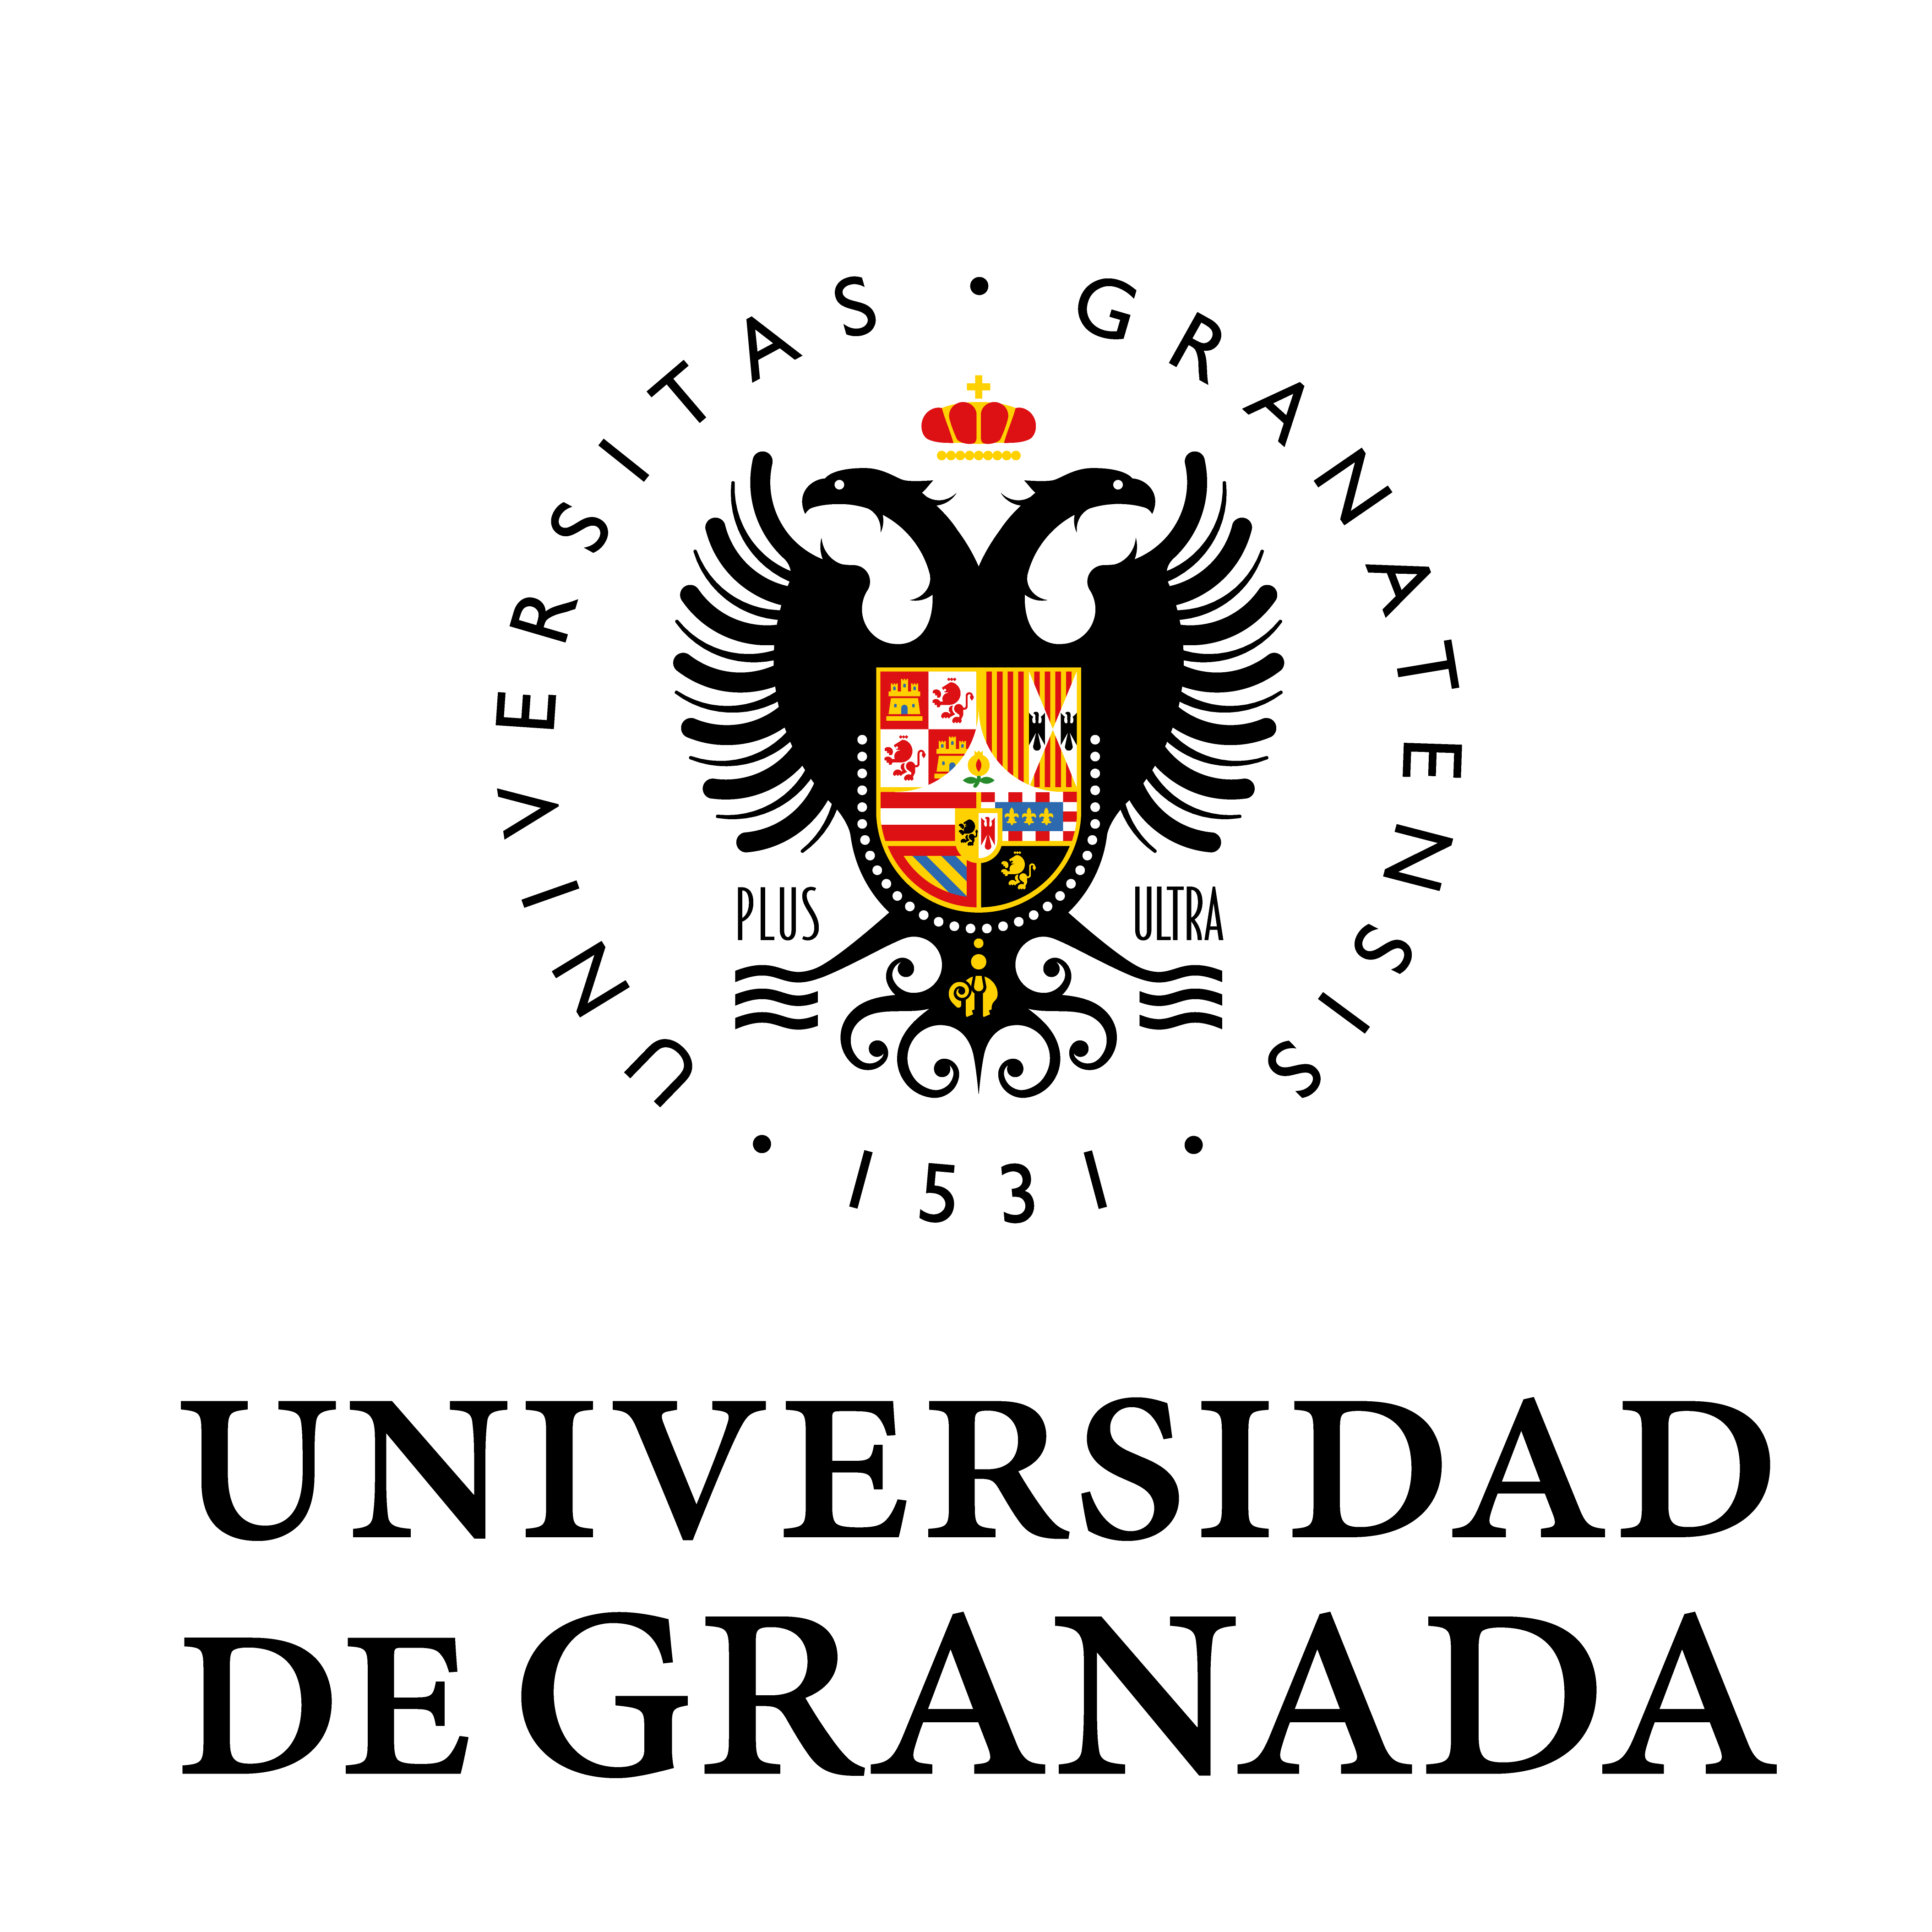
\includegraphics[width=0.7\textwidth]{logo.png}\par\vspace{1cm}
  {\scshape\large Sistemas Gráficos \par} \vspace{1cm}
  {\huge\bfseries Diseño e implementación de \\ un sistema gráfico \par}
  \vspace{0.4cm}
  {\large\bfseries ---Diseño---\\}
  \vspace{0.6cm}
  {\large\itshape  Guillermo Sandoval Schmidt  \par} \vspace{1.00cm}
  Curso 2019-2020 \\
  \vfill

  % Bottom of the page
  {\large 12 de junio de 2020 \par}
\end{titlepage}

\pagenumbering{gobble}
\pagenumbering{arabic}
\tableofcontents
\thispagestyle{empty}

\newpage

\section{Grupo de prácticas}
\begin{itemize}
    \item \textbf{Nombre de Alumno:} Guillermo Sandoval Schmidt
    \item \textbf{Nombre de la Aplicación:} Tetris
\end{itemize}

\section{Introducción}

La aplicación está basada en el juego popular juego 'TETRIS', creado en los años 80. La aplicación cuenta con dos partes claramente distinguibles. \\

La primera, la pantalla de inicio, dónde el jugador puede pulsar el botón PLAY usando su ratón para comenzar la partida, y que incluye dos animaciones, una en la que se mueve el título del juego y otra que genera varias piezas en posiciones aleatorias dentro de la pantalla y la atraviesan de arriba a abajo. La segunda, el juego, dónde el control pasa a ser por teclado y que incluye las diversas mecánicas de juego propias del mismo, información con el estado de la partida (nivel actual, siguiente pieza, puntuación, etc) y un recordatorio de los controles del juego.

\section{Clases}

    \subsection{Principales}
        \begin{itemize}
            \item \textbf{MyBoard:} está compuesto de 3 objetos de la clase \texttt{MyPiece} (pieza inicial, siguiente y guardada) y X*Y cubos de las clase \texttt{MyCube} que conforman el tablero. Se encarga de la gestión de las piezas y las colisiones de las mismas con el tablero. También gestiona todo lo relacionado con mecánicas del juego como el efecto de caída libre o el eliminar filas completas.
            \item \textbf{MyGame:} gestiona el texto y los valores relacionados con la putuación y otros parámetros auxiliares. También gestiona el comienzo de la partida y su fin, así como todas las animaciones \texttt{TWEEN} relacionadas con la partida en curso.
            \item \textbf{MyMenu:} está compuesto por un objeto de la clase \texttt{MyTitle}, con su animación propia, un objeto de la clase \texttt{MyKeyObj} que sirve como botón para comenzar la partida y varios objetos de la clase \texttt{MyPiece} con una animación que se encuentra más detallada en el apartado 6.1.
            \item \textbf{MyScene:} es la clase principal de la aplicación, gestionando los apartados propios de la escena como las cámaras, luces, la música, el cambio entre la pantalla de título y la partida y la captación de los diversos eventos tanto por teclado como por ratón. 
        \end{itemize}
    \subsection{Secundarias}
        \begin{itemize}
            \item \textbf{MyControls:} asemeja a un enumerado. En él se definen las teclas que se utilizan para los controles de las piezas de juego. Incluye un método que gestiona los movimientos, las rotaciones, el guardado de piezas o la caída directa de cada pieza (\textit{hard drop}).
            \item \textbf{MyKeyObj:} consta de dos objetos \texttt{MyRoundShape}, uno blanco, más grande, y otro negro, algo más pequeño y superpuesto por encima del blanco. La idea es crear una tecla sobre la que después se incluye texto con ayuda de \texttt{MyText:}. Se han implementado dos métodos, para poder llevar a cabo la selección del objeto y la deselección; consisten en un cambio de materiales en el objeto para que se pueda apreciar a simple vista que el botón ha sido pulsado o soltado.
            \item \textbf{MyPiece:} crea una pieza y la coloca en la posición indicada mediante los parámetros de la clase. Las piezas se generan de forma aleatoria y se construyen en consecuencia (hay distintas formas de piezas, y cada una tiene un material asociado). Las piezas se pueden mover por el tablero y también ser rotadas mediante los métodos \texttt{move} y \texttt{rotate}.
            \item \textbf{MyTitle:} crea el título del juego, tanto en la clase \texttt{MyMenu} y \texttt{MyBoard}. Para ello, depende de la clase auxiliar \texttt{MyText}. Recibe una posición y un tamaño para crearlo. La animación del texto se puede activar mediante un booleano, también argumento de la clase. Para dicha animación se utiliza \texttt{TWEEN}.
        \end{itemize} 
    
    \subsection{Auxiliares}
        \begin{itemize}
            \item \textbf{MyCube:} construye un cubo con las medidas, el material y la posición pasados como argumento.
            \item \textbf{MyMaterial:} es una clase que asemeja un enumerado de otros lenguajes. Contiene la declaración de los distintos materiales usados en la aplicación.
            \item \textbf{MyRoundShape:} crea una figura con las esquinas redondeadas que sirve de base para crear los botones y la pantalla de \textit{Game Over}.
            \item \textbf{MyText:} crea un objeto 3D con el texto que se le pasa como parámetro. Se indica también la posición, el material, el tamaño y la fuente utilizada.
        \end{itemize}
        
\newpage

\section{Diagrama de clases}

Debido al tamaño del diagrama de clases se ha decidido no incluir en el mismo las clases auxiliares. Incluso con este cambio, se recomienda visualizar el diagrama por separado, el cuál se incluye en la carpeta \texttt{doc}.\\

El diagrama resultante es el siguiente:

\begin{figure}[H]
    \centering
    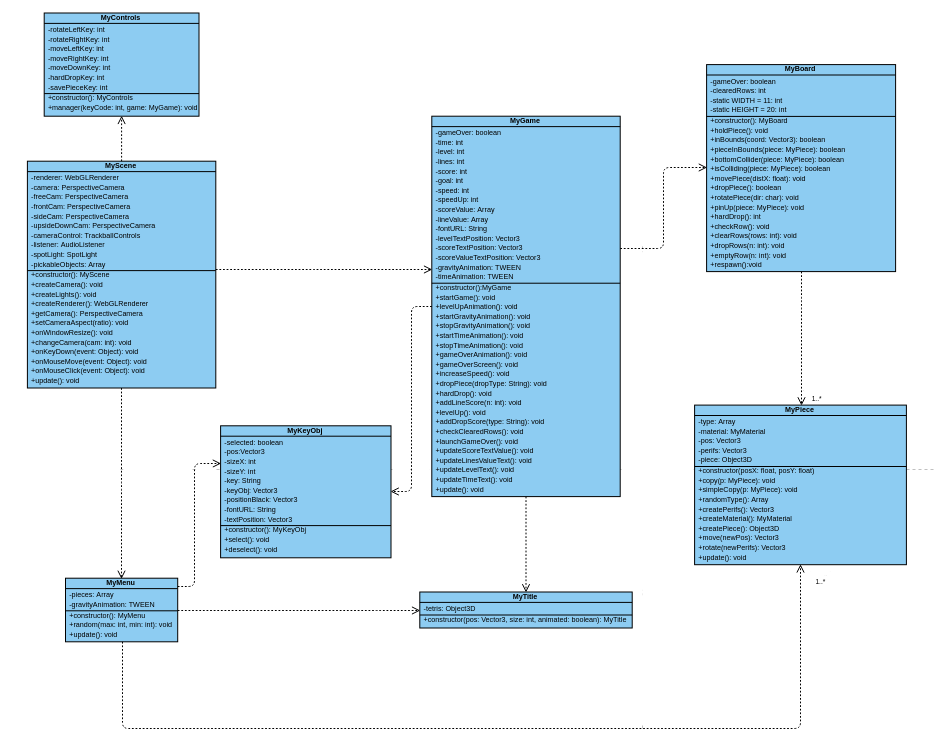
\includegraphics[scale=0.50]{diagrama.png}
    \caption{Diagrama de clases}
\end{figure}

\newpage

\section{Colisiones}

Respecto a las físicas y las colisiones podemos distinguir dos puntos importantes:
\begin{itemize}
    \item \textbf{Fronteras del tablero:} de cara a la detección de colisiones, se ha tenido en cuenta los límites laterales del tablero a la hora de mover o girar una pieza hacia la IZQUIERDA y la DERECHA y el límite inferior a la hora de mover la pieza hacia abajo o de que la mueva la gravedad implícita del juego, fijando la pieza en caso de colisionar con este límite.
    \item \textbf{Piezas inmóviles en el tablero:} de cara a la detección de colisiones, se ha tenido en cuenta las piezas que ya forman parte del tablero, no permitiendo que el jugador ocupe su posición al desplazar la pieza actual horizontalmente o al girarla y fijando la pieza en caso de colisionar desde la parte superior.
\end{itemize}

También se ha tenido en consideración tanto los diversos movimientos de la pieza (desplazamiento horizontal, desplazamiento hacia abajo, rotaciones, efecto 'caída libre') como la gravedad implícita en el juego, haciendo que aumente la velocidad con la que caen las piezas en función del nivel. Estos apartados se detallan en la siguiente sección.

\begin{figure}[H]
    \centering
    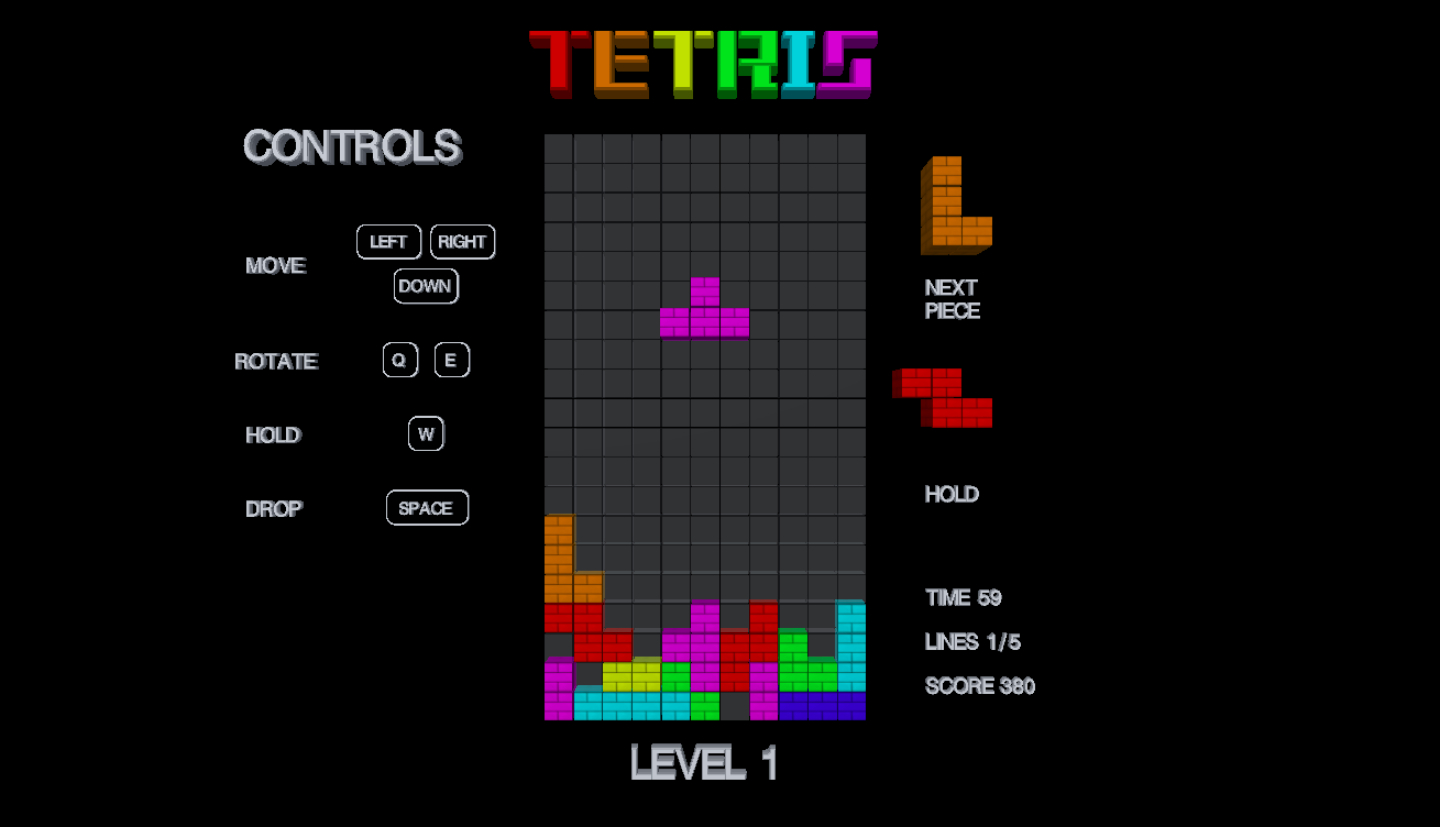
\includegraphics[scale=0.29]{game.jpg}
    \caption{Desarrollo de la partida}
\end{figure}

\newpage

\section{Animaciones}

    \subsection{Apartado de jugabilidad}
    \begin{itemize}
        \item \textbf{Gravedad:} se utiliza una animación \texttt{TWEEN} en bucle que hace que la pieza que controla el jugador caiga una casilla cada X tiempo, incrementando esta velocidad en función del nivel en el que nos encontremos.
        \item \textbf{Tiempo de juego:} se utiliza una animación \texttt{TWEEN} en bucle que modifica un parámetro \textit{time} y lo actualiza en pantalla.
        \item \textbf{Guardar pieza:} se activa mediante la interacción directa del jugador con el teclado, guardando la pieza actual y haciendo aparecer en el tablero la siguiente pieza o intercambiándola por la pieza guardada si ya tuviésemos una.
        \item \textbf{Mover pieza:} se activa mediante la interacción directa del jugador con el teclado, permitiendo desplazar la pieza actual una casilla hacia la IZQUIERDA o la DERECHA, respetando las limitaciones indicadas en la sección anterior.
        \item \textbf{Girar pieza:} se activa mediante la interacción directa del jugador con el teclado, permitiendo rotar la pieza actual hacia la IZQUIERDA o la DERECHA, respetando las limitaciones indicadas en la sección anterior.
         \item \textbf{Game Over:} se utilizan 4 animaciones \texttt{TWEEN}, una inicial que hará que una pantalla de \textit{GAME OVER} se sitúe en mitad de la pantalla del jugador que se encadena con otras 3 animaciones que retiran y los elementos \textit{TIME}, \textit{LINES} y \textit{SCORE}, introduciéndolos en la pantalla de \textit{GAME OVER}.
    \end{itemize}
    
    \begin{figure}[H]
        \centering
        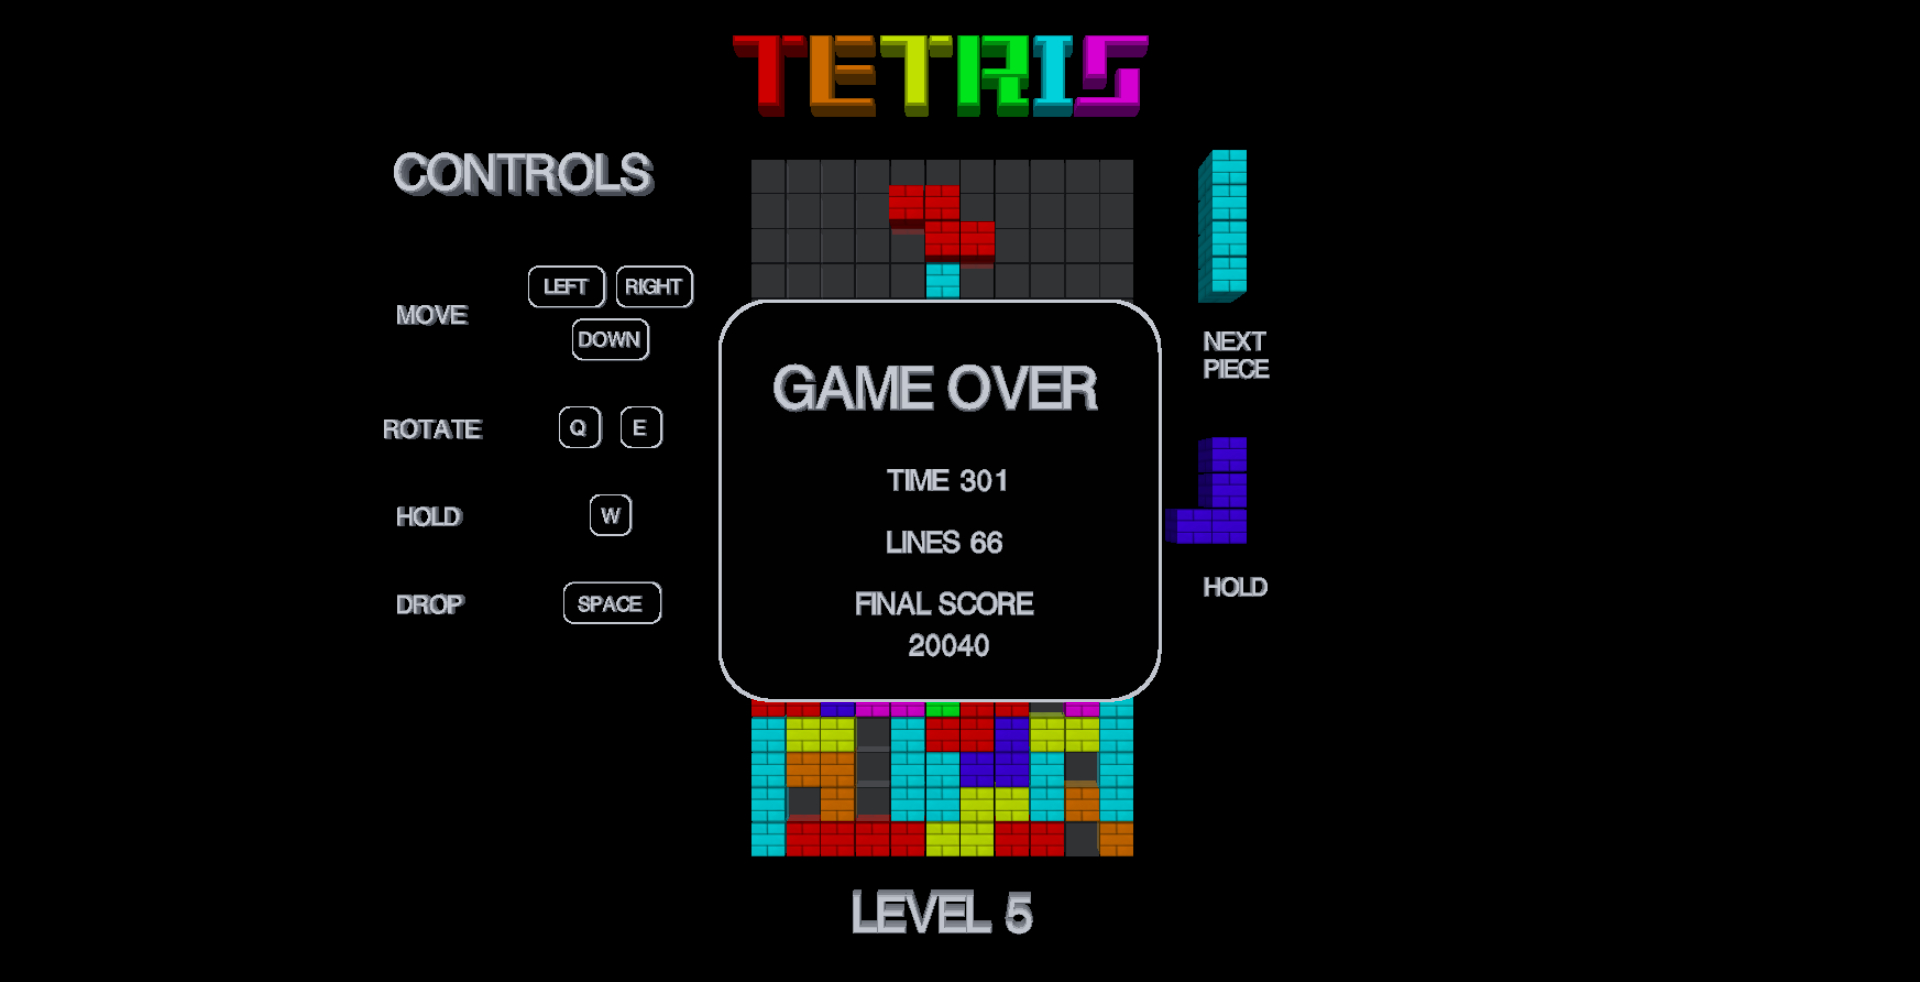
\includegraphics[scale=0.22]{gameOver.jpg}
        \caption{Pantalla de \textit{Game Over}}
    \end{figure}

    \subsection{Apartado estético}
    \begin{itemize}
        \item \textbf{Título del inicio:} se utilizan dos animaciones \texttt{TWEEN} para mover las letras de la palabras 'TETRIS' arriba y abajo, o efecto 'yoyo', animaciones que se pueden desactivar al crear el objeto de la clase \texttt{MyTitle}.
        \item \textbf{Piezas del inicio:} se utiliza una animación \texttt{TWEEN} que genera aleatoriamente (tanto el tipo de pieza como su posición en los ejes X y Z) y que desplaza varias piezas de arriba a abajo de la pantalla, en el eje Y, a distinta velocidad.
    \end{itemize}
    
    \begin{figure}[H]
        \centering
        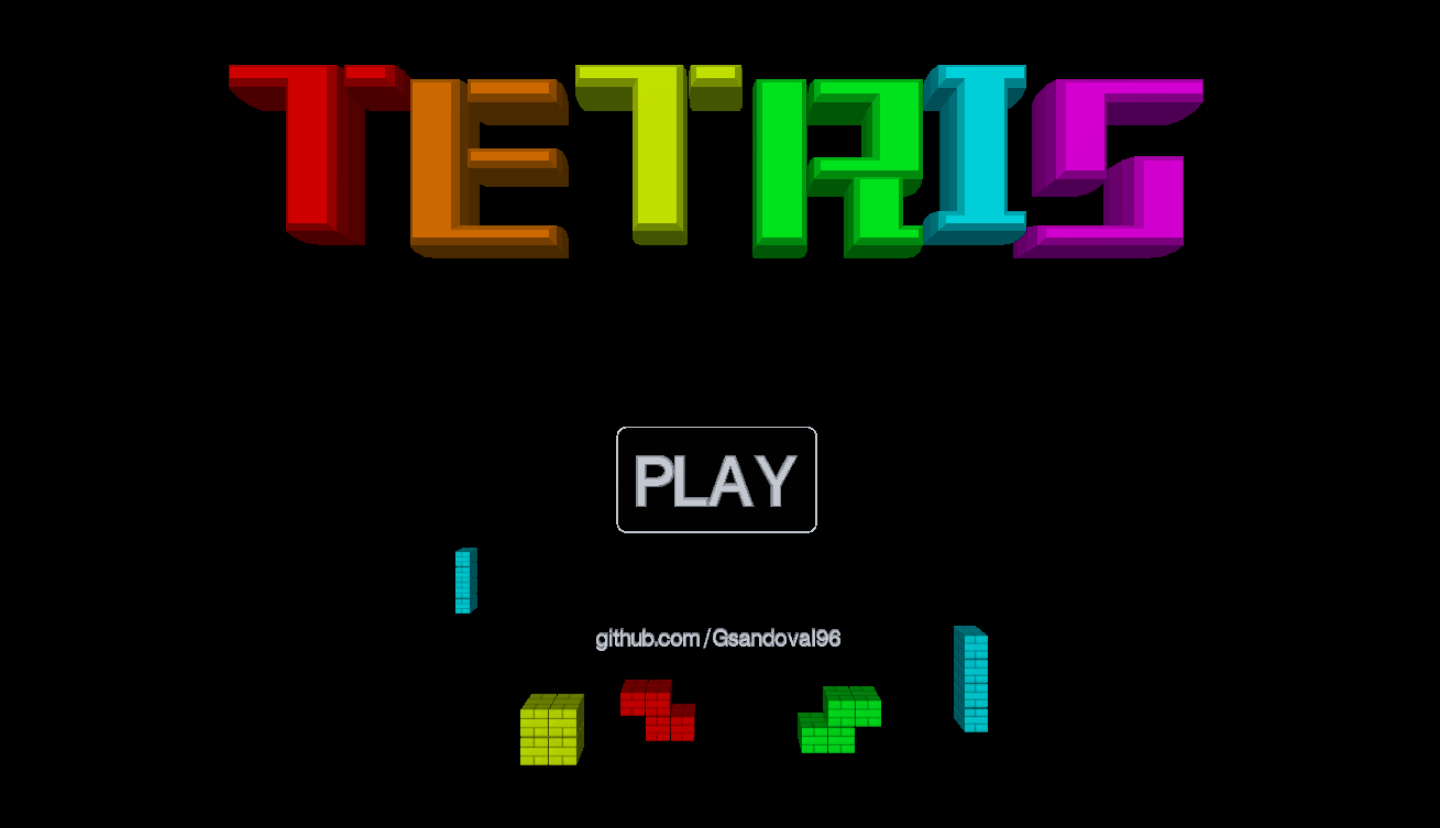
\includegraphics[scale=0.29]{menu.jpg}
        \caption{Menú de inicio}
    \end{figure}
    
\section{Otros elementos}

    \subsection{Materiales y texturas}
    
    Para los materiales se ha creado la clase \texttt{MyMaterial} que incluye todos los materiales utilizados en el proyecto. Se ha escogido el tipo de material \href{https://threejs.org/docs/#api/en/materials/MeshStandardMaterial}{MeshStandardMaterial} debido a que nos ofrece un aspecto más realista que otros materiales de la biblioteca.\\
    
    Para las texturas se han incluido materiales con textura de ladrillo para su uso en las piezas del Tetris.
    
    \subsection{Luces}
     
     Se utiliza una luz simple tipo \href{https://threejs.org/docs/#api/en/lights/SpotLight}{SpotLight} de color BLANCO y situada alejada en el eje Z y ligeramente inclinada respecto al centro de la escena para visualizar bien las sombras generadas en los objetos de la misma. También se ha incluido una luz ambiental tipo \href{https://threejs.org/docs/#api/en/lights/AmbientLight}{AmbientLight}.
        
    \subsection{Música}
    
    Para la música se han usado las clases \href{https://threejs.org/docs/#api/en/audio/Audio}{Audio}, \href{https://threejs.org/docs/#api/en/loaders/AudioLoader}{AudioLoader} y \href{https://threejs.org/docs/#api/en/audio/AudioListener}{AudioListener}, cargandola e iniciandola al comienzo y activando el modo de reproducción en bucle.
    
    \subsection{Cámaras}
    
    Todo lo relacionado con las cámaras se puede consultar en el Manual de Usuario, disponible en la carpeta \texttt{doc}.
    
    \subsection{Interacción}
    
    Todo lo relacionado con la interacción de usuario con la aplicación y los controles se puede consultar en el Manual de Usuario, disponible en la carpeta \texttt{doc}.

\section{Github}

Todo el proyecto y el código se encuentra disponible en: \href{https://github.com/Gsandoval96/SG-UGR/tree/master/P2}{github.com/Gsandoval96/SG-UGR}, dónde se puede consultar todo el proceso realizado mediantes los commits del respositorio.

\section{Bibliografía}

\begin{itemize}
    \item \textbf{Documentación} 
    \begin{itemize}
        \item Documentación y ejemplos de three.js disponible en \href{https://threejs.org/}{https://threejs.org/}.
        \item Material de la asignatura Sistemas Gráficos, impartida por el profesor D. Francisco Velasco Anguita.
    \end{itemize}
    \item \textbf{Material}
    \begin{itemize}
        \item Fuentes en formato .json generadas con: \href{http://gero3.github.io/facetype.js/}{Facetype.js}.
        \item Música descargada de: \href{https://downloads.khinsider.com/game-soundtracks/album/tetris-99-original-soundtrack}{https://downloads.khinsider.com}.
    \end{itemize}
    \item\textbf{Herramientas}
        \begin{itemize}
            
            \item Texturas diseñadas con la herramienta online: \href{https://www.photopea.com/}{Photopea}.
            \item Diagrama de clases realizado con la herramienta online: \href{https://online.visual-paradigm.com/es/}{Online Visual-Paradigm}
        \end{itemize}
    
\end{itemize}

\end{document}
